%% Basierend auf einer TeXnicCenter-Vorlage von Mark Müller
%%%%%%%%%%%%%%%%%%%%%%%%%%%%%%%%%%%%%%%%%%%%%%%%%%%%%%%%%%%%%%%%%%%%%%%

% Wählen Sie die Optionen aus, indem Sie % vor der Option entfernen  
% Dokumentation des KOMA-Script-Packets: scrguide

%%%%%%%%%%%%%%%%%%%%%%%%%%%%%%%%%%%%%%%%%%%%%%%%%%%%%%%%%%%%%%%%%%%%%%%
%% Optionen zum Layout des Artikels                                  %%
%%%%%%%%%%%%%%%%%%%%%%%%%%%%%%%%%%%%%%%%%%%%%%%%%%%%%%%%%%%%%%%%%%%%%%%
\documentclass[%
%a5paper,							% alle weiteren Papierformat einstellbar
%landscape,						% Querformat
%10pt,								% Schriftgröße (12pt, 11pt (Standard))
%BCOR1cm,							% Bindekorrektur, bspw. 1 cm
%DIVcalc,							% führt die Satzspiegelberechnung neu aus
%											  s. scrguide 2.4
%twoside,							% Doppelseiten
%twocolumn,						% zweispaltiger Satz
%halfparskip*,				% Absatzformatierung s. scrguide 3.1
%headsepline,					% Trennline zum Seitenkopf	
%footsepline,					% Trennline zum Seitenfuß
%titlepage,						% Titelei auf eigener Seite
%normalheadings,			% Überschriften etwas kleiner (smallheadings)
%idxtotoc,						% Index im Inhaltsverzeichnis
%liststotoc,					% Abb.- und Tab.verzeichnis im Inhalt
%bibtotoc,						% Literaturverzeichnis im Inhalt
%abstracton,					% Überschrift über der Zusammenfassung an	
%leqno,   						% Nummerierung von Gleichungen links
%fleqn,								% Ausgabe von Gleichungen linksbündig
%draft								% überlangen Zeilen in Ausgabe gekennzeichnet
]
{scrartcl}

%\pagestyle{empty}		% keine Kopf und Fußzeile (k. Seitenzahl)
%\pagestyle{headings}	% lebender Kolumnentitel

%% Deutsche Anpassungen %%%%%%%%%%%%%%%%%%%%%%%%%%%%%%%%%%%%%
\usepackage[english]{babel}
\usepackage[T1]{fontenc}
\usepackage[utf8]{inputenc}

\usepackage{amsthm} % Theorem-Packet
\usepackage{amsmath}
\usepackage{amssymb}

\usepackage{stmaryrd} % Blitzsymbol
\usepackage{fancyhdr} % Für Kopfzeile
\usepackage{graphicx} % Einbinden von Grafiken
\usepackage{bbding} % Für das Häckchen
\usepackage{amscd} % Kommutative Diagramme
\usepackage{mathtools} % Für das Definitionssymbol

\usepackage{listings}
\usepackage{courier}

\pagestyle{fancy}
\lhead{Computational Science I}\chead{Exercise notes: Markov and Newton-Cotes}\rhead{HS 2013} % Kopfzeile

\newtheoremstyle{plain}%  name
  {.5\baselineskip}% Space above
  {.5\baselineskip}% Space below
  {}% Body font
  {}% Indent amount (empty = no indent, \parindent = para indent)
  {\bfseries}% Thm head font
  {:}% Punctuation after thm head
  { }% Space after thm head: " " = normal interword space; \newline = linebreak
  {}% Thm head spec (can be left empty, meaning `normal')
  
\makeatletter % Matrizen mit opitonalen Linien
\renewcommand*\env@matrix[1][*\c@MaxMatrixCols c]{%
  \hskip -\arraycolsep
  \let\@ifnextchar\new@ifnextchar
  \array{#1}}
\makeatother

\theoremstyle{plain}
\newtheorem*{bsp}{Beispiel} % Beispiele ohne Nummerierung
\newtheorem*{bws}{Beweis} % Beweise ohne Nummerierung 
\newenvironment{beweis}{\begin{bws}~\vspace{0.5\baselineskip}}{\hfill $\qedsymbol$\end{bws}}
\newenvironment{beispiel}{\begin{bsp}~\vspace{0.5\baselineskip}}{\end{bsp}}

\usepackage{lmodern} % Type1-Schriftart für nicht-englische Texte

\usepackage{enumerate}

\renewcommand\theenumi{\roman{enumi}}
\renewcommand\labelenumi{\theenumi)}

%% Packages für Grafiken & Abbildungen %%%%%%%%%%%%%%%%%%%%%%
%\usepackage{graphicx} %%Zum Laden von Grafiken
%\usepackage{subfig} %%Teilabbildungen in einer Abbildung
%\usepackage{tikz} %%Vektorgrafiken aus LaTeX heraus erstellen

%\setlength{\parindent}{0pt} % kein Einzug


%% Beachten Sie:
%% Die Einbindung einer Grafik erfolgt mit \includegraphics{Dateiname}
%% bzw. über den Dialog im Einfügen-Menü.
%% 
%% Im Modus "LaTeX => PDF" können Sie u.a. folgende Grafikformate verwenden:
%%   .jpg  .png  .pdf  .mps
%% 
%% In den Modi "LaTeX => DVI", "LaTeX => PS" und "LaTeX => PS => PDF"
%% können Sie u.a. folgende Grafikformate verwenden:
%%   .eps  .ps  .bmp  .pict  .pntg


%% Bibliographiestil %%%%%%%%%%%%%%%%%%%%%%%%%%%%%%%%%%%%%%%%%%%%%%%%%%
%\usepackage{natbib}

\begin{document}

\lstset{basicstyle=\ttfamily, breakatwhitespace=false, breaklines=true, frame=single, xleftmargin=\parindent, aboveskip=\baselineskip, belowskip=\baselineskip}

%\pagestyle{empty} %%Keine Kopf-/Fusszeilen auf den ersten Seiten.


%%%%%%%%%%%%%%%%%%%%%%%%%%%%%%%%%%%%%%%%%%%%%%%%%%%%%%%%%%%%%%%%%%%%%%%
%% Ihr Artikel                                                       %%
%%%%%%%%%%%%%%%%%%%%%%%%%%%%%%%%%%%%%%%%%%%%%%%%%%%%%%%%%%%%%%%%%%%%%%%

%% eigene Titelseitengestaltung %%%%%%%%%%%%%%%%%%%%%%%%%%%%%%%%%%%%%%%    
%\begin{titlepage}
%Einsetzen der TXC Vorlage "Deckblatt" möglich
%\end{titlepage}

%% Angaben zur Standardformatierung des Titels %%%%%%%%%%%%%%%%%%%%%%%%
\titlehead{\center{University of Zurich - HS 2013}}
%\subject{Typisierung}
\title{Computational Science I\\Exercise notes:  Markov and Newton-Cotes\\\rule{1.0\textwidth}{1.0pt}}
\author{Tobias Grubenmann}
%\and{Der Name des Co-Autoren}
%\thanks{Fußnote}			% entspr. \footnote im Fließtext
%\date{}							% falls anderes, als das aktuelle gewünscht
%\publishers{Herausgeber}

%% Widmungsseite %%%%%%%%%%%%%%%%%%%%%%%%%%%%%%%%%%%%%%%%%%%%%%%%%%%%%%
%\dedication{Widmung}

\maketitle 						% Titelei wird erzeugt

%% Zusammenfassung nach Titel, vor Inhaltsverzeichnis %%%%%%%%%%%%%%%%%
%\begin{abstract}
% Für eine kurze Zusammenfassung des folgenden Artikels.
% Für die Überschrift s. \documentclass[abstracton].
%\end{abstract}

%% Erzeugung von Verzeichnissen %%%%%%%%%%%%%%%%%%%%%%%%%%%%%%%%%%%%%%%
%\tableofcontents			% Inhaltsverzeichnis
%\listoftables				% Tabellenverzeichnis
%\listoffigures				% Abbildungsverzeichnis


%% Der Text %%%%%%%%%%%%%%%%%%%%%%%%%%%%%%%%%%%%%%%%%%%%%%%%%%%%%%%%%%%

\section*{Exercise 1}

The simulation of lighthouse flashes runs 500 times with $a=-0,5$ and $b=0.7$. Only the values for $x$ between -1 and 1 are stored into a list, all others are ignored.

After the simulation, the Metropolis algorithm runs with 1000 Iterations trying to recover $a$ and $b$. For this purpose the joint probability for random values for $a$ and $b$ is calculated over all $x$. The new parameters $a$ and $b$ are accepted if the quotient between the new and the old joint probability is greater than a random value from a uniform $[0,1]$ distribution:

\lstinputlisting[language=Python]{../Lighthouse.py}

The histogram of random flashes and of the parameters $a$ and $b$ are as following:

\begin{center}
\centering
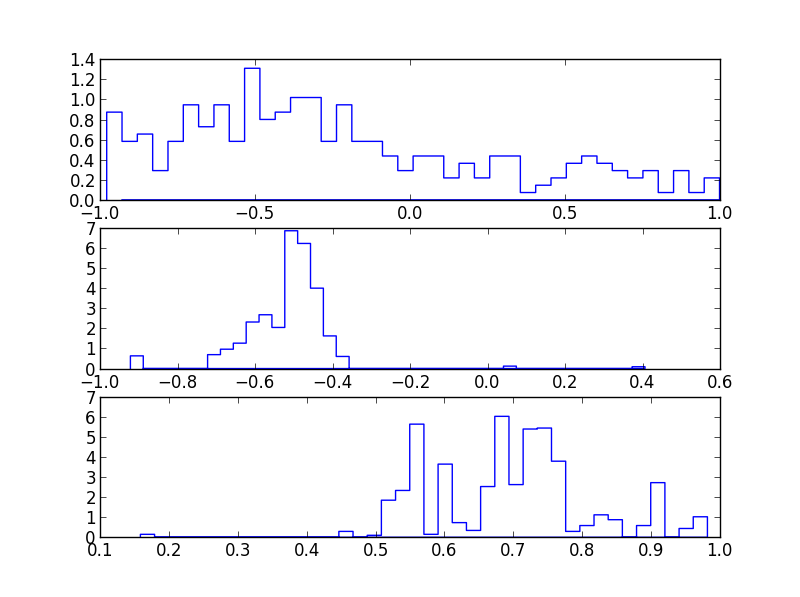
\includegraphics[width=0.6\linewidth]{../Lighthouse.png}
\captionof{figure}{Lighthouse with 500 flashes, $a=-0.5$, $b=0.7$}
\end{center}

\section*{Exercise 1}

By the symmetry of the integration rule the polynomials $x$,$x^{3}$ and $x^{5}$ are always integrated correctly. Therefore, we only have to consider the polynomials $1$, $x^{2}$ and $x^{4}$. Now,

\begin{eqnarray*}
\int\limits_{-5}^{5}1dx&=&\left[x\right]^{5}_{-5}=2\cdot 5\\
\int\limits_{-5}^{5}x^{2}dx&=&\left[\frac{1}{3}x^{3}\right]^{5}_{-5}=2\cdot\frac{1}{3}5^{3}\\
\int\limits_{-5}^{5}x^{4}dx&=&\left[\frac{1}{5}x^{5}\right]^{5}_{-5}=2\cdot\frac{1}{5}5^{5}
\end{eqnarray*}

With this values, we can build a system of linear equations:

\begin{equation*}
\begin{pmatrix}\frac{1}{2}&1&1\\0&2^{2}&4^{2}\\0&2^{4}&4^{4}\end{pmatrix}\begin{pmatrix}c_{0}\\c_{2}\\c_{4}\end{pmatrix}=\begin{pmatrix}5\\\frac{1}{3}5^{3}\\\frac{1}{5}5^{5}\end{pmatrix}
\end{equation*}

The following Python script solves the equation above and then derives the coefficients as fractions:

\lstinputlisting[language=Python]{../5PointIntegrator.py}

The solution for the coefficients is:

\begin{eqnarray*}
c_{0}&=&\frac{335}{96}\\
c_{2}&=&\frac{125}{144}\\
c_{4}&=&\frac{1375}{576}
\end{eqnarray*}

\section*{Exercise 3}

The function \texttt{fivepoint( f , a, b, B = 1)} approximates the integral of $f$ between $a$ and $b$ using $B$ blocks using the five point rule derived from the last exercise:

\lstinputlisting[language=Python]{../FivePoint.py}

To calculate $\int\limits_{-\infty}^{+\infty}e^{-x^{2}}dx$ I use the following transform of variables:

\begin{eqnarray*}
x&=&\frac{t}{1-t^{2}}\\
\frac{dx}{dt}&=&\frac{(1-t^{2})+2t^{2}}{(1-t^{2})^{2}}=\frac{1+t^{2}}{(1-t^{2})^{2}}
\end{eqnarray*}

We can now rewrite the integral:

\begin{equation*}
\int\limits_{-\infty}^{+\infty}e^{-x^{2}}dx=\int\limits_{-1}^{1}e^{-\left(\frac{t}{1-t^{2}}\right)^{2}}\frac{1+t^{2}}{(1-t^{2})^{2}}dt
\end{equation*}

Using the above \texttt{fivepoint} function the integral evaluates to $1.7724538509059757\approx\sqrt{\pi}$.

%% Bibliographie unter Verwendung von dinnat %%%%%%%%%%%%%%%%%%%%%%%%%%
%\setbibpreamble{Präambel}		% Text vor dem Verzeichnis
%\bibliographystyle{dinat}
%\bibliography{bibliographie}	% Sie benötigen einen *.bib-Datei

\end{document}
